% This is "sig-alternate.tex" V2.0 May 2012
% This file should be compiled with V2.5 of "sig-alternate.cls" May 2012
%
% This example file demonstrates the use of the 'sig-alternate.cls'
% V2.5 LaTeX2e document class file. It is for those submitting
% articles to ACM Conference Proceedings WHO DO NOT WISH TO
% STRICTLY ADHERE TO THE SIGS (PUBS-BOARD-ENDORSED) STYLE.
% The 'sig-alternate.cls' file will produce a similar-looking,
% albeit, 'tighter' paper resulting in, invariably, fewer pages.
%
% ----------------------------------------------------------------------------------------------------------------
% This .tex file (and associated .cls V2.5) produces:
%       1) The Permission Statement
%       2) The Conference (location) Info information
%       3) The Copyright Line with ACM data
%       4) NO page numbers
%
% as against the acm_proc_article-sp.cls file which
% DOES NOT produce 1) thru' 3) above.
%
% Using 'sig-alternate.cls' you have control, however, from within
% the source .tex file, over both the CopyrightYear
% (defaulted to 200X) and the ACM Copyright Data
% (defaulted to X-XXXXX-XX-X/XX/XX).
% e.g.
% \CopyrightYear{2007} will cause 2007 to appear in the copyright line.
% \crdata{0-12345-67-8/90/12} will cause 0-12345-67-8/90/12 to appear in the copyright line.
%
% ---------------------------------------------------------------------------------------------------------------
% This .tex source is an example which *does* use
% the .bib file (from which the .bbl file % is produced).
% REMEMBER HOWEVER: After having produced the .bbl file,
% and prior to final submission, you *NEED* to 'insert'
% your .bbl file into your source .tex file so as to provide
% ONE 'self-contained' source file.
%
% ================= IF YOU HAVE QUESTIONS =======================
% Questions regarding the SIGS styles, SIGS policies and
% procedures, Conferences etc. should be sent to
% Adrienne Griscti (griscti@acm.org)
%
% Technical questions _only_ to
% Gerald Murray (murray@hq.acm.org)
% ===============================================================
%
% For tracking purposes - this is V2.0 - May 2012

%Englisch: Kommentar hier entfernen
\documentclass{sig-alternate}
%Deutsch: Kommentar hier entfernen
%\documentclass{sig-alternate-de}

\begin{document}
%
% --- Author Metadata here ---
\conferenceinfo{Advances in Embedded Interactive Systems}{'14 Passau, Germany}
\CopyrightYear{2014} % Allows default copyright year (20XX) to be over-ridden - IF NEED BE.
%\crdata{0-12345-67-8/90/01}  % Allows default copyright data (0-89791-88-6/97/05) to be over-ridden - IF NEED BE.
% --- End of Author Metadata ---

\title{Traffic Flow Optimization via Connected Cars}
%
% You need the command \numberofauthors to handle the 'placement
% and alignment' of the authors beneath the title.
%
% For aesthetic reasons, we recommend 'three authors at a time'
% i.e. three 'name/affiliation blocks' be placed beneath the title.
%
% NOTE: You are NOT restricted in how many 'rows' of
% "name/affiliations" may appear. We just ask that you restrict
% the number of 'columns' to three.
%
% Because of the available 'opening page real-estate'
% we ask you to refrain from putting more than six authors
% (two rows with three columns) beneath the article title.
% More than six makes the first-page appear very cluttered indeed.
%
% Use the \alignauthor commands to handle the names
% and affiliations for an 'aesthetic maximum' of six authors.
% Add names, affiliations, addresses for
% the seventh etc. author(s) as the argument for the
% \additionalauthors command.
% These 'additional authors' will be output/set for you
% without further effort on your part as the last section in
% the body of your article BEFORE References or any Appendices.

\numberofauthors{1} %  in this sample file, there are a *total*
% of EIGHT authors. SIX appear on the 'first-page' (for formatting
% reasons) and the remaining two appear in the \additionalauthors section.
%
\author{
% You can go ahead and credit any number of authors here,
% e.g. one 'row of three' or two rows (consisting of one row of three
% and a second row of one, two or three).
%
% The command \alignauthor (no curly braces needed) should
% precede each author name, affiliation/snail-mail address and
% e-mail address. Additionally, tag each line of
% affiliation/address with \affaddr, and tag the
% e-mail address with \email.
%
% 1st. author
\alignauthor
Thomas Leutheusser\\
       \affaddr{Universität Passau}\\
       \affaddr{Lehrstuhl für Informatik mit Schwerpunkt Eingebettete Systeme}\\
       \affaddr{Innstr. 43}\\
       \affaddr{94032 Passau, Germany}\\
       \email{leutheus@fim.uni-passau.de}
}
% There's nothing stopping you putting the seventh, eighth, etc.
% author on the opening page (as the 'third row') but we ask,
% for aesthetic reasons that you place these 'additional authors'
% in the \additional authors block, viz.

\date{22 November 2014}
% Just remember to make sure that the TOTAL number of authors
% is the number that will appear on the first page PLUS the
% number that will appear in the \additionalauthors section.

\maketitle
\begin{abstract}

\end{abstract}

\keywords{}

\section{Introduction}
Upcoming technology of connected vehicles hitting consumer market soon (TODO: Quelle finden). What are ITS. Overview of benefits of ITS especially as a measure against traffic congestion, reduced travel times and resulting reduction of emissions.
\section{Traffic Flow Optimization }
The main parameters of traffic flow have to be quantified in order to evaluate and compare different traffic flows. Including others these parameters consist of speed, flow, density, mean speed, and headway. Flow describes the rate at which vehicles pass a fixed point in a time interval. Density is the concentration of vehicles over a fixed length of a roadway. Mean speed is divided into time mean speed, which is the arithmetic mean of vehicle speeds passing a point, and space mean speed, which is the harmonic mean of speeds passing a point during a period of time. The headway is the time that elapses between a vehicle and a following vehicle passing a certain point. \\
Traffic flow can be analyzed at three different levels of granularity. Microscopic traffic flow examines individual vehicles and their properties like speed and position. Macroscopic scale investigates traffic flow characteristics such as density, flow and mean speed on a traffic stream. Mesoscopic models allow the study of large areas with applications such as congestion relief through alternative routes. \\
As a result the types of traffic flow optimization can be applied to different types of granularity. \\
Microscopic optimizations focus on improving the mean travel time for single vehicles by finding optimal vehicle TODO actions actions such as finding the optimal lane or adjusting the speed to decrease the amount of brake/accelerations actions. These optimizations are discussed in chapter TODO\\
The goal of macroscopic optimizations is the increase of throughput and reduced travel times for a given traffic stream. They are discussed in section TODO \\
Mesoscopic optimizations are briefly mentioned in section TODO\\

\subsection{Microscopic Traffic Flow Optimizations}
\subsubsection{Optimal Lane Selection}
One driving behavior that can heavily interrupt the flow of traffic are lane changes. The need for lane changes derives from the inequality of desired driving speeds and mandatory lane changes like lane drops or exiting the current road. These lane changes may disrupt the traffic by aggressive maneuvers (i.e. cutting into small gaps). This papers TODO shows that lane changes disrupt the flow by creating a moving bottleneck under congested traffic conditions TODO cite quelle 3 des papers. \\
Jin et al.\cite{6856515} propose a cooperative real-time lane selection algorithm in which connected vehicles share information to improve the system-wide operation of traffic. Well-coordinated lane changes can help maintain desired speeds and minimize shock wave impacts.  [Zitat Seite 71 Absatz 3] \\
This is achieved by calculating the optimal lane target for each vehicle based on its location, speed, lane and desired driving speed. These parameters are transmitted from each car to a roadside communication unit (RSU) which can exchange these real-time information within a certain range. The RSU calculates the optimal lane for each vehicle and sends its optimal lane advice. \\
Jin et al.\cite{6856515} tested the algorithm on a simulated 3-way highway of 2000m length with one roadside communication unit with 300 meters communication range and connected vehicles with a speed of 50 mp/h using the microscopic simulation tool SUMO\cite{sumo}.In the simulation, the mean travel times of different road congestion levels (50\%, 60\%, ... 100\%) with and without their proposed algorithm were compared. Besides the mean travel times, the reduction of energy consumption and the emission of pollutants was simulated (CO, HC, NOx, PM2.5) with MOVES\cite{simulator2010user} (Motor Vehicle Emission Simulator).\\
The simulated mean travel time was reduced by 0,57\% at 50\% road congestion, up to 3.79\% improvement (118.4s to 115.3s) at 70\% of the maximum density. At higher congestion levels the vehicles could not always find the needed space in their suggested lanes, which reduces the success rate of a lane change. At a level of 0.95\% of the maximum capacity of the road, an improvement of 2.67\% in mean travel times was still detected. \\
Similar to the travel times the reduction in pollutants peaked at 70\% road congestion. Energy consumption and CO2 emissions are reduced by around 2.2\% while CO and HC emissions are reduced by up to 17\%. Jin et al. demonstrate how connected vehicles can improve the traffic flow through microscopic actions like well coordinated lane changes. However they do not take into account different penetration rates of interconnected vehicles, which could be useful for the transition years between current and next generation cars. They only simulate their algorithm on a 3-way highway with relatively low speed limit (50mp/h) and equally treated vehicles. Different simulation runs with trucks, or 2-way highways and  varying penetration rates of V2x technology could have given more insights into the usefulness of this approach. 
\subsubsection{Lane drop merging assistance}
The second microscopic optimization next to optimal lane changes is the coordinated approach to a lane drop. Schuhmacher et al.\cite{1614269.1614274} provide a Merging assistance algorithm which advices drivers on the individual speed limits and merging positions ahead of a lane drop. The current traffic control strategies in front of lane drop consist of
\begin{description}
\item[Gradual speed limit reduction] Usually used at highway lane drops. The speed limit in front of a lane merge is decreased in several stages to achieve a harmonization of traffic with decreased frictions between vehicles and an increased traffic safety.
\item[Late merge strategy] Drivers are advised to stay in their lane up to the lane drop. This allows the usage of all available lanes until the lane drop. This strategy performs particularly well with heavily congested traffic and low speeds. 
\item [Early merge strategy] Warning signs indicating the lane drop are placed far ahead encouraging the drivers to switch the lane early. This reduces forced merges in the vicinity of the drop. This strategy is preferred at low traffic demands with higher speeds.  
\end{description} 

Schuhmacher et al. present a method which reduces traffic jams and increases capacity in front of a lane drop by switching to a more effective strategy with the usage of car-to-x communication for controlled merging procedures.\\ The reference scenario is based on an empiric study\cite{bertini2005empirical} of a freeway lane drop between Heathrow and London, where the passing lane of a 3-way highway transitions to two lanes. The length of the sections and the placement of traffic detectors can be seen in Figure \ref{fig:schuhmacher1} which was taken from \cite {1614269.1614274}. \\
\begin{figure} [h]
\centering
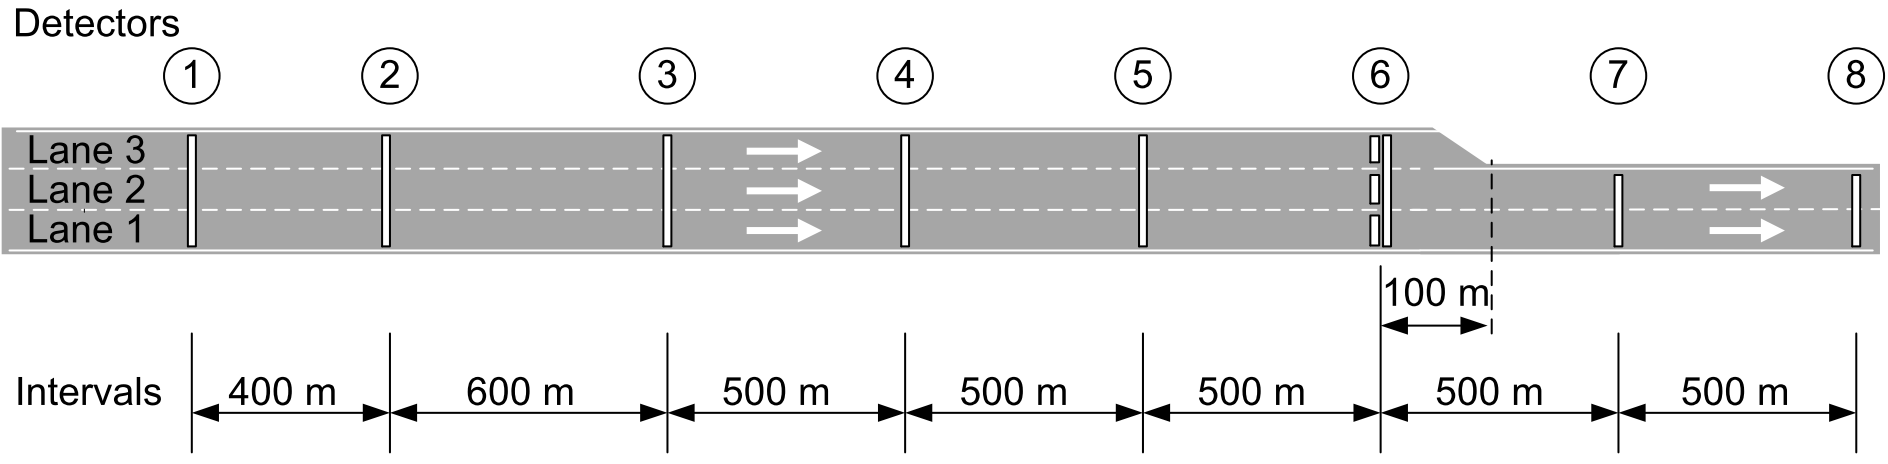
\epsfig{file=schuhmacher_1.png, height=1in, width=3.3in}
\caption{Reference scenario map with distance intervals}
\label{fig:schuhmacher1}
\end{figure}
Their approach uses a Road-side Unit (RSU) 350m in front of the lane drop (between detector 5 and 6 of Figure \ref{fig:schuhmacher1}) and On-board units (OBUs) in the vehicles to allow the communication of traffic control messages. The communication parameters are chosen with respect to the IEEE 802.11 family of standards and the 802.11p amendment for Wireless Access in Vehicular Environments (WAVE). Specifically the RSU and OBUs communication range is set to 500 metres. The OBUs are aware of their position (e.g. through GPS) and can not only receive messages from the RSU but also forward messages to other OBUs to achieve a multi-hop communication. \\
The implementation of the merging assistance is a combination of dynamic merge strategies and dynamic gradual speed limits. The main part of the merging assistance algorithmn is implemented in the RSU. It analyzes the current traffic conditions by monitoring the time mean speeds of vehicles at the detectors and transmitting traffic control messages  to the OBUs accordingly. These messages consist of the gradual speed limit, the merging positions (e.g. at which point in front of the lane drop the lane switch should occur) and additional messages as "Stay in Lane"  for upstream vehicles and special  "Do Not Pass" messages for heavy vehicles after the merge point, which reduces frictions during the merge procedure as no heavy vehicles are permitted on the lane being merged to. \\
The algorithmn works in different stages based on the time mean speed TMS of vehicles at detectors 5 and 6 (the two in front of the lane drop). The TMS are re-evaluated every 5 seconds.
$v_5$ and $v_6$ describe the TMS of detector 5 and 6 respectively. DEM stands for Dynamic Early Merge, DLM for Dynamic Late Merge.
\begin{description}
\item[DEM Stage 1] $v_6 > 80 km/h$ \\
The traffic directly in front of the lane drop (at detector 6) is flowing freely with speeds over 80 km/h. The merge point is set to 400m in front of the lane drop and a no passing zone for heavy vehicles 400 m ahead of the lane drop is established. 
\item[DEM Stage 2] $v_6<= 80 km/h$ and $v_5>80 km/h$ \\ 
The TMS reduction at detector 6 indicates increasing traffic density resulting in merging problems and braking vehicles. To counteract the merging point is shifted 400m upstream to a distance of 800m to the lane drop. Ahead of it a "Stay in Lane" zone is established. After it the "Do not pass" rule for heavy vehicles apply. In addition the gradual speed limit reduction is applied to 110, 100, 90 km/h at distances of 2500, 2000, 1000 m ahead of the lane drop, respectively. 
\item[DEM Stage 3] $60 km/h < v_6 <= 80 km/h$ \\ and $v_5 <= 80 km/h$\\
The slightly congested area with decreased TMS between 60 and 80 km/h extended up to detector 5. The distance of the merging point and the "Stay in Lane" zone ahead of it is set to 1300m. Heavy vehicles are not allowed to pass after the merge point. Gradual speed limit is at 100/90/80 km/h at 2500, 2000, 1000 m.
\item [DLM] $v_6 <= 60 km /h$ \\
Under 60 km/h TMS the traffic condition is assumed to be heavily congested. At this stage it is more efficient to use all lanes as long as possible to maximize the capacity. The merge point is shifted to 100 m ahead of the lane drop, with the "Stay in Lane" and "Do not pass" zones adjusted accordingly. The speed limits are reduced to 90,70,60 km/h at 2500, 2000, 1000 m, respectively.
\end{description}

Schuhmacher et al. simulated their algorithm and the reference scenario with the AIMSUN \footnote{$http://www.aimsun.com/wp/?page\_id=21$} traffic simulator. 
The maximum capacity of a lane was set to 2000 vehicles per hour. The proportion of heavy vehicles was set to 15\% and the maximum allowed speed is 112km/h (70 mp/h).
%\begin{table}
%\centering
%\caption{reference scenario traffic demand}
%\begin{tabular}{l|c} 
%\textbf{time} & \textbf{traffic demand}  \\ \hline
%0 - 60 min & 3100 veh/min \\ \hline
%60 - 120 min & 5000 veh/min \\ 
%
%\end{tabular}
%
%\end{table}

\subsection{Macroscopic Optimization}
\subsubsection{Adaptive Traffic Lights}

\subsection{Mesoscopic Optimization}
\subsubsection{Route guidance}
\section{Discussion}

\section{Conclusion}



%%%%%%%%%%%%%%%%%%%%

\section{Erster Entwurf veraltet}

What is traffic flow optimiziation. What is needed for Traffic flow optimization (Traffic detection?) Traffic Prediction \cite{6856591}. \\ How to achieve optimization Self-organization?\cite{5625236} \\Overview of next subsections Traffic Control with its subsubsections Traffic Lights and Traffic Management Systems. \\
Economic Driving: Improvements such as reduction of emissions via V2V communication.  \\
Can V2V  improve traffic?  Yes example\cite{6856462}
\subsection{Traffic Control}
Real-time lane selection\cite{6856515} \\
Speed control at lane drop \cite{1614269.1614274}\\
Noch ein zusätzliches Paper finden\\
\subsubsection{Virtual and Adaptive Traffic Lights}
In-vehicle virtual traffic lights\cite{ferreira2010self}  \cite{gradinescu2007adaptive} \\ 
Dynamic lane grouping \cite{6338840} \\
Dynamic traffic lights with emergency/high priority vehicles \cite{6799827} \\
\subsubsection{Route Guidance and Traffic Management Systems}
Traffic Prediction Models \cite{6685576} \\
Graphical Route Guidance \cite{5410169} \\
Vanet based route guidance \cite{6799873}
Finding optimal routes through traffic with v2v  find paper \\
Navigation System paper finden\\
\subsection{Economic Driving}
V2V communication helps reducing emissions. find more papers \\
Optimal trajectory and brake/acceleration \cite{6856456} 
\subsection{Discussion and Comparison} Compare methods discuss benefits and disadvantages.
\subsection{Conclusions}
Improvement through usage of v2v communication. 
%\end{document}  % This is where a 'short' article might terminate

%ACKNOWLEDGMENTS are optional
\subsection{Acknowledgments}


%
% The following two commands are all you need in the
% initial runs of your .tex file to
% produce the bibliography for the citations in your paper.
% ENGLISCH: Kommentar dieser Zeile entfernen
\bibliographystyle{abbrv}
% DEUTSCH: Kommentar dieser Zeile entfernen
%\bibliographystyle{abbrv-de}
\bibliography{bibliography}  % bibliography.bib is the name of the Bibliography in this case
% You must have a proper ".bib" file
%  and remember to run:
% latex bibtex latex latex
% to resolve all references
%
% ACM needs 'a single self-contained file'!
%
%APPENDICES are optional
%\balancecolumns

% This next section command marks the start of

%\balancecolumns % GM June 2007
% That's all folks!
\end{document}
